\section{Code Transformation for Distributed Training}\label{sec:trans}
\subsection{Python Abstract Syntax}\label{sec:pysyn}

(Describe the simplified Python abstract syntax here. 
The abstract syntax should be sufficient to describe our code transformation. 
We can attach the full Python abstract syntax as supplementary material.)

We first define the abstract syntax for Python programming language.
The syntax of Python is described in the Python Language Reference \cite{pythonref}.
The reference provides a full grammar specification based on the extended PEG,
and detailed explanation of syntatic components in each section.
We manually examined the grammar and the details
to define the Python abstract sytax.
The syntax is composed of three syntactic components: expressions, statements,
and top-level components.

Expressions are parts of the code that evaluates to a value.
Python has 5 kinds of primitive values, 
which are numbers, strings, booleans, the value 'None' and 'Ellipsis'.
The value 'None' is used to denote a undefined value,
similar to the value `null` in Java.
The value 'Ellipsis' corresponds to the notation "...",
which can be used as an special placeholder meaning expansion of the sequence. 
Python has composite types of tuple, list, set, map, and custom classes.
The expression syntax defines ways to build up values
and complex expressions such as operators, comprehension, and function calls. 

Statements are parts of the code that changes the program state,
such as variable binding or control flow. 
Python statements are categorized into 
simple statements which denote a single state changing step, 
or compound statements which are composed of multiple statements.

Simple statements include assignment statements and import statements.
Assignment statements are used to declare a new variable and its value
or update a variable value.
Import statements are used to specify a module, load it
and get definitions of the module into current namespace.
In import statements, each target module and its aliased name is represented
as alias. (...TODO:insert alias abstract syntax...)  
Note that procedure call is a special case of expression statements,
where the expression is a function call.

Compound statements include conditional statements, loop statements,
and definitions for functions and classes.
Additionally, the with statement is an special kind of compound statement.
With statement is identical to the assignment statement 
in a way that it binds an expression to a name, 
but the statement additionally adds implicit calls
to the object's methods related to initialization and destruction.
Similar to the alias in import statement,
with statements use WithItem to represent then ame and expression.
(...TODO:insert WithItem abstract syntax...) 

Top-level components are representation of the program
in different execution environment of the Python interpreter.
For example, a module represents a Python code file, composed of
multiple definitions speicified of statements. 
The full Python abstract syntax is attched in the supplementary material.

\subsection{Training API Patterns for TensorFlow ML model}

(introduce what we describe here, and why it is needed.)
We categorized TensorFlow ML models by patterns of training API usage.

(explain pattern by pattern with examples)

\subsection{Transformation Rule for Distributed TensorFlow ML model}

In this section, we describe the transformation rule that
transforms single-GPU based TensorFlow model codes into
multi-GPU based TensorFlow model codes.
We informally understand code transformation rule as
conditions to select the target code parts
and methods to actually transform them into another.
The methods include addition, modification, and deletion of
specific code parts.
Currently, code transformation for distributed ML training
is only described by set of examples and informal explanations.
In order to automate the code transformation process,
we need to formally define the code transformation rule
and ways to convert the definition into software implementation.
We propose a formal definition of code transformation rule
for distributed ML training, and implement the automatic code transformation
software based on the formal definition.

Code transformation is formally defined as a pure function from AST to AST.
AST is an abbreviation of abstract syntax trees; it is a tree data structure
that represents grammatical structure of the program code.
We call this function a transform function.
We may define multiple transform functions that act on different kinds
of AST and use them to define other transform functions.
For example, in order to transform a Python code into another,
we define a transform function that takes Module AST and returns Module AST.
Inside the Module transform function definition,
we may use Statement transform function to transform statements
that compose the Module AST.

Together with the AST parameter, transform functions take and return
the environment parameter.
Environment parameters are used to store specific identifiers
and pass it to the other calls of the transform function.
For example, statement transform function frequently use 
the identifier bound to the TensorFlow module.
The module name first appears from the import statement.
The transform function call on the import statement stores
the TensorFlow module name on the environment and returns it.
Then the later function calls to other statements can
retrieve the TensorFlow module name from the environment parameter.

We define the transform function in terms of pattern matching on input AST.
The pattern matching is used to match the kind and content of the input AST
and construct an output AST.

(TODO figure of transforming AST of the statement below
optimizer = tf.keras.optimizers.Adam(lr)
optimizer = tf.keras.optimziers.Adam(lr * hvd.size())
)

The above figure illustrates the example of a statement transformation.
Intutitive understanding of the transformation is as follows:
if the input code is assignment statment 
that assigns a new 'tf.keras.optimizer.Adam' instance,
then multiply 'hvd.size()' on learning rate argument expression of the
instance constructor function.
The transform function should describe two aspects of the sentence;
first it should describe the condition of "assignment statement that
creates 'tf.keras.optimizer.Adam' instance";
second it should describe the transformation sentence
of "multiply 'hvd.size()' on the learning rate argument". 

(TODO figure of part of transform function describing the example) 

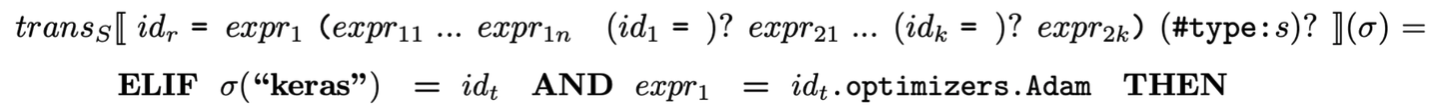
\includegraphics[width=15cm]{trans_ex01}

The figure defines the part of Statement transform function. 
The pattern matched by the function is described on the first line;
it matches the assignment statements with operator '=' and
right-hand side of function call expression.
Note that the input AST components are matched onto pattern variables.
This allows the definition to reuse the input AST component
when constructing the output AST.
The second line illustrates pattern guard that matches the input AST content.
It checks the callee expression is the expression 'tf.keras.optimizers.Adam'.
The pattern guard uses the environment parameter $\sigma$ to retrieve
module name for the Keras module.

(TODO figure of part of transformation function deescribing example,
output only. remove the keyword args case)

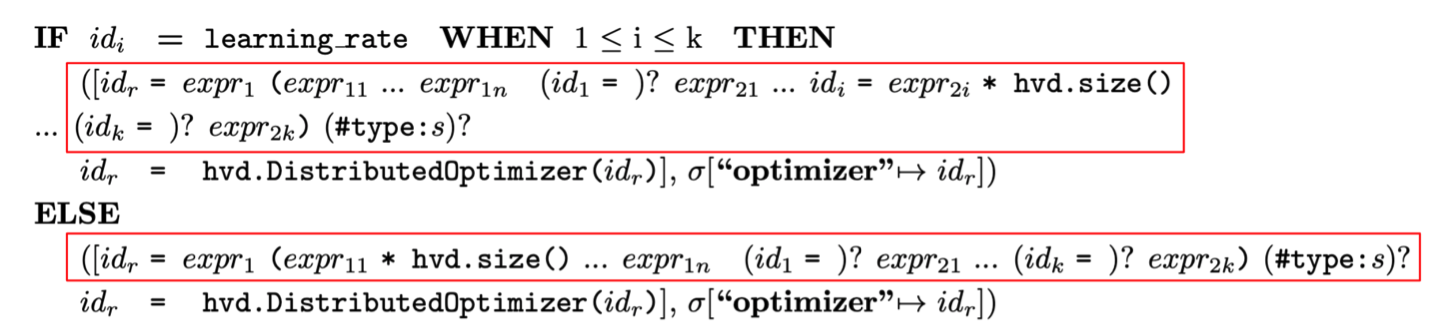
\includegraphics[width=15cm]{trans_ex02}

The figure defines the following part of the function.
It describes the construction of an output AST and environment.
The output AST is assignment statement which
the right-hand side function argument expression is modified.
As previously mentioned, the construction use pattern matched variables
to reuse the input AST components.
The difference is that first argument expression is multiplied by 'hvd.size()',
which formally describes the transformation sentence.

We inspected multiple references to define the whole transform function.
Horovod documentation\cite{horovodtf} describes the code modification
required to change trainig script. It describes six steps to modify
existing training scripts to distributed training scripts. 
In addition to 

\subsection{...}
Describe how to transform TensorFlow ML models to training them on distributed
systems with the horovod framework. We can use formal rules we defined and some
code examples here. We can attach the full transformation rules as
supplementary material as well.  Please write this and some more following
subsections to describe the transformation.
